\chapter{Conclusion}
brief of conclusion

\section{Annisa Fathoroni/1164067}
\subsection{Teori}
Penjelasan Tugas Harian 9 ( No 1-6 )
\begin{enumerate}
\item Mengapa Kata-Kata Harus Di Lakukan Vektorisasi Dan Ilustrasi Gambar.
\begin{itemize}
\item Penjelasan:

Karenakan mesin hanya mampu membaca data dengan bentuk angka.Berdasarkan hal tersebut maka tentunya diperlukan vektorisasi kata atau bisa disebut dengan mengubah kata menjadi bentuk vektor agar mesin seolah-olah paham apa yang kita maksudkan dan dapat memproses aktifitas/perintah dengan benar. Selain alasan diatas, kata harus di vektorisasiuntuk mengetahui presentase kata yang sering muncul dalam setiap kalimatnya, yang berguna untuk menetukan kata kunci.

\item Ilustrasi Gambar

\begin{figure}[!hbtp]
\centering
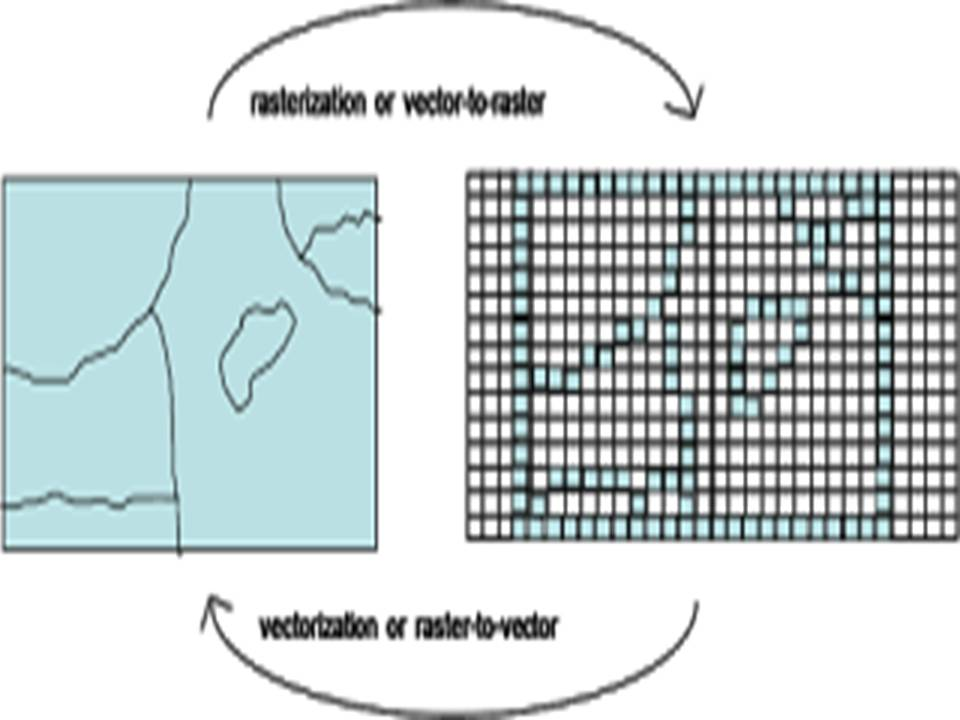
\includegraphics[scale=0.3]{figures/Chapter5AnnisaFathoroni5.jpg}
\caption{Vektorisasi - Annisa Fathoroni}
\label{Vektorisasi - Annisa Fathoroni}
\end{figure}

\end{itemize}

\item Mengapa Dimensi Dari Vektor Dataset Google Bisa Mencapai 300 Dan Ilustrasi Gambar.
\begin{itemize}
\item Penjelasan:

Karena pada masing-masing objek yang terdapat pada dataset akan memiliki identitasnya tersendiri. Apabila dicontohkan dengan penjelasan yang lebih rinci maka dilakukan perumpamaan sederhana. Misalnya untuk sebuah dataset google yang memiliki 3 buah objek yaitu berat, lebar, dan tinggi.  Kemudian dari masing-masing objek tersebut dilakukan perbandingan antara berat dan lebar beserta berat dan tinggi. Hasil yang didapatkan akan memiliki presentasi yang berbeda sehingga dapat diartikan bahwa mesin dapat membedakan objek yang hampir serupa namun tak sama.

\item Ilustrasi Gambar

\begin{figure}[!hbtp]
\centering
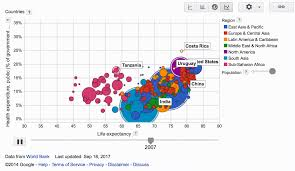
\includegraphics[scale=0.8]{figures/Chapter5AnnisaFathoroni7.jpg}
\caption{Dimensi Vektor Dataset - Annisa Fathoroni}
\label{Dimensi Vektor Dataset - Annisa Fathoroni}
\end{figure}

\end{itemize}

\item Konsep Vektorisasi Untuk Kata Dan Ilustrasi Gambar.
\begin{itemize}
\item  Penjelasan:

Konsep untuk vektorisasi kata sebenarnya sama dengan ketika dilakukan input suatu kata pada mesin pencarian. Kemudian untuk hasilnya akan mengeluarkan ( berupa ) referensi mengenai kata tersebut. Jadi data kata tersebut didapatkan dari hasil pengolahan pada kalimat-kalimat sebelumnya yang telah diolah. Contoh sederhananya pada kalimat berikut ( Please click the alarm icon for more notifications about my channel ), pada kalimat tersebut terdapat konteks yakni channel, kata tersebut akan dijadikan data latih untuk mesin yang akan dipelajari dan diproses. Jadi ketika kita inputkan kta channel, maka mesin akan menampilkan keterkaitannya dengan kata tersebut sehingga akan lebih efisien dan lebih mudah.

\item Ilustrasi Gambar

\begin{figure}[!hbtp]
\centering
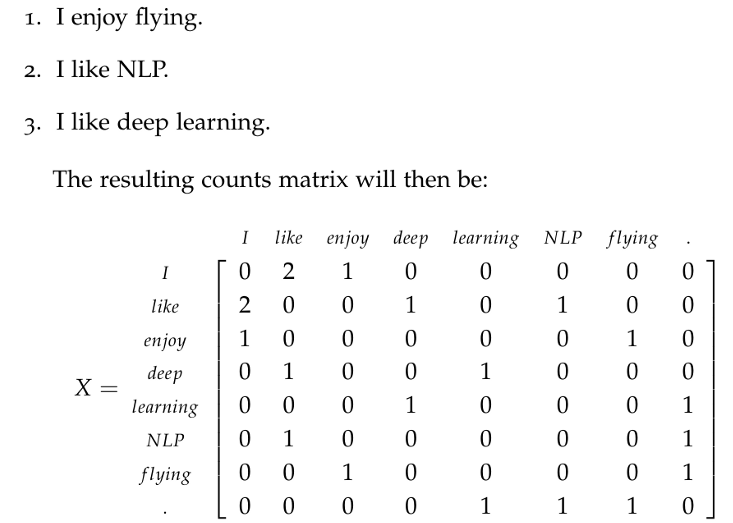
\includegraphics[scale=0.5]{figures/Chapter5AnnisaFathoroni4.png}
\caption{Vektorisasi Untuk Kata - Annisa Fathoroni}
\label{Vektorisasi Untuk Kata - Annisa Fathoroni}
\end{figure}

\end{itemize}

\item Konsep Vektorisasi Untuk Dokumen Dan Ilustrasi Gambar.
\begin{itemize}
\item  Penjelasan:

Untuk vektorisasi dokumen sebenarnya terbilang sama dengan konsep vektorisasi kata, yang membedakan hanya pada proses awalnya ( pada eksekusi awal ). Untuk vektorisasi dokumen ini, mesin akan membaca semua kalimat yang terdapat pada dokumen tersebut, kemudian kalimat yang terdapat pada dokumen tersebut akan di pecah menjadi kata-kata. Seperti itulah konsep vektorisasi dokumen.

\item Ilustrasi Gambar

\begin{figure}[!hbtp]
\centering
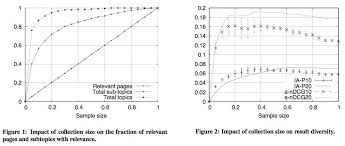
\includegraphics[scale=0.8]{figures/Chapter5AnnisaFathoroni6.jpg}
\caption{Vektorisasi Untuk Dokumen - Annisa Fathoroni}
\label{Vektorisasi Untuk Dokumen - Annisa Fathoroni}
\end{figure}

\end{itemize}

\item Pengertian Mean Dan Standar Devisiasi Beserta Ilustrasi Gambar.
\begin{itemize}
\item  Pengertian Mean:

Mean adalah nilai rata-rata dari beberapa buah data. Nilai mean dapat ditentukan dengan membagi jumlah data dengan banyaknya data. Mean (rata-rata) merupakan suatu ukuran pemusatan data. Mean suatu data juga merupakan statistik karena mampu menggambarkan bahwa data tersebut berada pada kisaran mean data tersebut. Mean tidak dapat digunakan sebagai ukuran pemusatan untuk jenis data nominal dan ordinal.

\item  Pengertian Standar Devisiasi:

Standar Deviasi dan Varians Salah satu teknik statistik yg digunakan untuk menjelaskan homogenitas kelompok. Varians merupakan jumlah kuadrat semua deviasi nilai-nilai individual thd rata-rata kelompok. Sedangkan akar dari varians disebut dengan standar deviasi atau simpangan baku. Standar Deviasi dan Varians Simpangan baku merupakan variasi sebaran data. Semakin kecil nilai sebarannya berarti variasi nilai data makin sama Jika sebarannya bernilai 0, maka nilai semua datanya adalah sama. Semakin besar nilai sebarannya berarti data semakin bervariasi.

\item Ilustrasi Gambar

\begin{figure}[!hbtp]
\centering
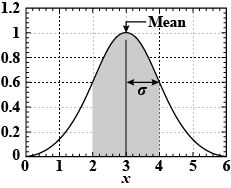
\includegraphics[scale=0.7]{figures/Chapter5AnnisaFathoroni2.png}
\caption{Mean - Annisa Fathoroni}
\label{Mean - Annisa Fathoroni}
\end{figure}

\begin{figure}[!hbtp]
\centering
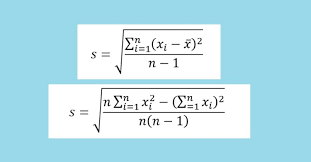
\includegraphics[scale=0.7]{figures/Chapter5AnnisaFathoroni3.png}
\caption{Standar Devisiasi - Annisa Fathoroni}
\label{Standar Devisiasi - Annisa Fathoroni}
\end{figure}

\end{itemize}

\item Penjelasan Skip-gram Dan Ilustrasi Gambar
\begin{itemize}
\item  Penjelasan:

Skip-Gram adalah kebalikannya, yaitu mencoba memprediksi vektor kata-kata yang ada di konteks diberikan vektor kata tertentu. Skip-Gram membuat sepasang kata target dan konteks sebagai sebuah instance sehingga Skip-Gram cenderung lebih baik ketika ukuran corpus sangat besar. 

\item Ilustrasi Gambar

\begin{figure}[!hbtp]
\centering
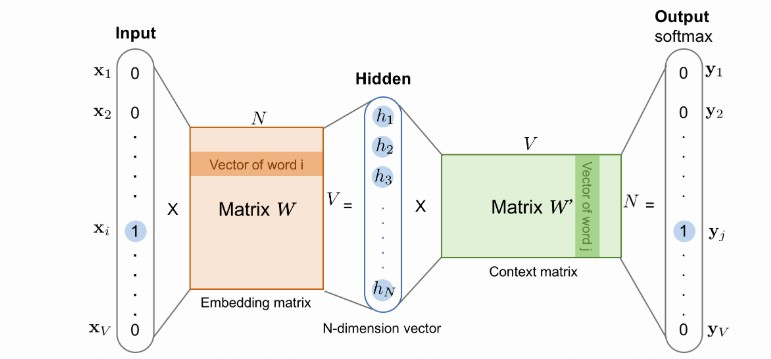
\includegraphics[scale=0.5]{figures/Chapter5AnnisaFathoroni1.jpg}
\caption{Skip Gram - Annisa Fathoroni}
\label{Skip Gram - Annisa Fathoroni}
\end{figure}
\par
\par
\end{itemize}
\par
\par
\end{enumerate}


\section{Tasya Wiendhyra /1164086}
HARI PERTAMA MINGGU KELIMA

\subsection{Kenapa Kata-Kata Harus Di Lakukan Vektorisasi Beserta Ilustrasi}
Karena ketika menggunakan algoritma machine learning tidak bisa  secara langsung menggunakan teks melainkan teks tersebut harus diubah menjadi angka. Kita membutuhkan cara untuk merepresentasikan data teks untuk algoritma pembelajaran mesin, vektorirasi membantu mengubah teks biasa kedalam bentuk vektor yang dapat dimengerti oleh komputer atau machine learning. Kita mungkin ingin melakukan klasifikasi dokumen, sehingga setiap dokumen adalah "input" dan label kelas adalah "output" untuk algoritma prediksinyai. Algoritma mengambil vektor angka sebagai input, oleh karena itu kita perlu mengkonversi dokumen menjadi vektor angka dengan panjang tetap atau sama.
\par Untuk ilustrasinya misal,  saya memiliki kamus berisikan kata-kata {MonkeyLearn, is, not, great}, dan saya ingin membuat vektor teks "MonkeyLearn is great", saya akan memiliki vektor berikut: (1, 1, 0, 0, 1,) .

\subsection{Mengapa Dimensi Dari Vektor Dataset Google Bisa Sampai 300 Beserta Ilustrasi}
Karena di dalam satu dataset berisikan setidaknya 3 Milyar kata dan kalimat. Yang dimana dimensi berisikan kata - kata unik dari data tersebut. Maka dari itu dimensi pada dataset Google bisa mencapai 300.

Untuk ilustrasinya, misalkan kita memiliki sebuah buku dengan tebal 1000 , dimana bukunya dibagi menjadi dua Chapter. Kemudian kita akan menggabungkan kata dari setiap Chapter tersebut. Maka akan didapatkan irisan yang akan berjumlah lebih dari 200. dikarenakan banyak kata yang berbeda beda.

\subsection{Konsep Vektorisasi Untuk Kata}
Konsepnya yaitu kata atau teks akan dihapuskan noisy datanya atau dihapus data yang tidak terpakai, seperti tag html jika ada, titik, koma, dll. Kemudian tokenization artinya kita akan mengelompokan kalimat menjadi token atua membagi kata kata menjadi potingan kecil. Baru setelah itu dilakukan normalisasi untuk mengubah datanya menjadi angka.

Ilustrasinya, misalnya ada beberapa kalimat seperti berikut :
\begin{itemize}
\item There used to be Iron Age.

Kemudian didapatkan token seperti berikut “There”,”was”,”to”,”be”,”used”,”Stone”,”Bronze,”Iron”,”Revolution”,”Digital”,”Age”,”of”,”Now”,”it”,”is”

Maka ketika di cek pada kalimat diatas hasilya seperti berikut 
\item There used to be iron age = [1,0,1,1,1,0,0,1,0,0,1,0,0,0,0]
\end{itemize}

\subsection{Konsep Vektorisasi Untuk Dokumen}
Hampir mirip dengan konsep kata, namun untuk di dokumen biasanya konsepnya digunakan untuk mencari kesamaan atau memprediksi seberapa sering menculan kata dalam 2 kalimat atau 2 paragraf.

Ilustrasinya, misalkan dalam sebuah artikel kita ingin mencari seberapa banyak kata "dimana" muncul. Maka dengan Doc2Vec dapat diprediksi hasilnya.

\subsection{Mean Dan Standar Deviasi}
\subsubsection{Pengertian}
Mean adalah nilai rata-rata dari beberapa buah data. Nilai mean dapat ditentukan dengan membagi jumlah data dengan banyaknya data.

Deviasi standar adalah ukuran ringkasan perbedaan setiap pengamatan dari rata-rata. Deviasi standar mengukur penyebaran data tentang nilai rata-rata. Ini berguna dalam membandingkan set data yang mungkin memiliki mean yang sama tetapi rentang yang berbeda.

\subsubsection{Contoh}
\begin{enumerate}
\item Misalkan kita sudah menghitung tinggi anjing.
\begin{figure}[ht]
\centering
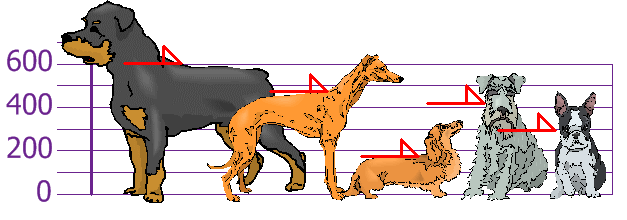
\includegraphics[scale=0.5]{figures/chapter5tasya1.png}
\caption{Contoh Mean dan Standar Deviasi }
\label{Teori}
\end{figure}
\item Tingginya dilihat dari bahu : 600mm, 470mm, 170mm, 430mm and 300mm.
\item Kita hitung mean atau rata ratanya, dengan menjumlahkan seluruh data dan membaginya dengan jumlah n nya hasilnya yaitu 394.
\item Kemudian kita ingin melihat berapa perbedaan tinggi dari anjing - anjing tersebut menggunakan variance. 
\item Baru Gunakan standar deviasi didapatkan hasil 147 mm . DEngan Deviasi Standar kita bisa tahau mana anjing dengan tinggi normal dan anjing yang kekurangan tinggi.
\begin{figure}[ht]
\centering
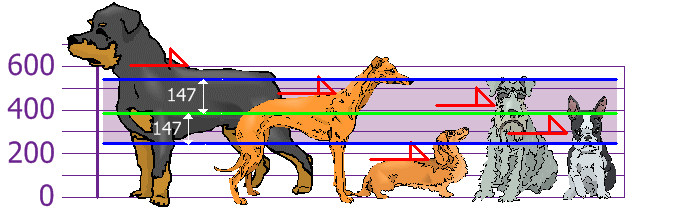
\includegraphics[scale=0.5]{figures/chapter5tasya2.png}
\caption{Contoh Mean dan Standar Deviasi }
\label{Teori}
\end{figure}

\subsection{Skip-gram}
Arsitektur model Skip-gram biasanya  mencoba untuk memprediksi kata konteks sumber (kata-kata sekitarnya) diberi kata target (kata tengah). Contohnya seperti berikut 
\begin{figure}[ht]
\centering
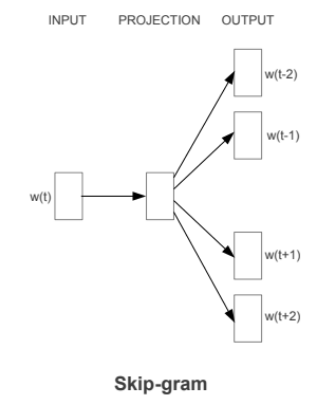
\includegraphics[scale=0.5]{figures/chapter5tasya3.png}
\caption{Contoh Skipgram }
\label{Teori}
\end{figure}
\end{enumerate}